
\section{MCS Performance on Simulated Single Muons}\label{singlemuon_MC_section}

% Executive summary
In this section, MCS performance is studied on a sample of simulated, fully contained, single muons in {\ub}. This section of the technote will include studies from this single muon sample with {\sc MCTracks} (described in Section \ref{MCTrack_section}).\\

It is demonstrated that the range-based momentum of a track agrees with the true momentum with negligible bias and with a resolution of better than 5\%. The MCS performance on single {\sc MCTracks} is shown to be comparable to that on single reconstructed PandoraNuPMA tracks when the track is well reconstructed, with a minimal bias and a resolution that varies between 2 and 10\%, performing better for higher momentum (longer) tracks. Additionally, the scattering angle of track segments for a given momentum is shown to be gaussian for {\sc MCTracks}, in line with the Highland formula prediction.


\subsection{Input Sample}\label{SingleMu_Input_Sample_section}
In order to study MCS performance in the most straightforward way, a sample of simulated single muons is used. This sample was generated in the {\ub} MCC7 production under the SAM definition ``prod\_muminus\_0-2.0GeV\_isotropic\_uboone\_mcc7\_reco2''. This sample consists of 19,500 single muons generated at a random location within the {\ub} TPC, with random direction. The energy spectrum of this sample is flat between 0 to 2 GeV kinetic energy of the muons. It is worth noting that the MCC7 simulation includes broken wires by masking specific channels on some planes in an attempt to better match real detector conditions, however {\sc MCTracks} are unaffected by this (Section \ref{MCTrack_section}).\\

% and with reconstructed tracks (described in Section \ref{RecoTrack_section}).

\subsection{Fiducial Volume Definition}\label{fidvol_section}
The {\ub} TPC has active volume dimensions of 2.6 m width $\times$ 2.3 m height $\times$ 10.4 m length. For this analysis, a smaller ``fiducial volume'' is defined and referenced throughout this note (for example, in many cases reconstructed tracks are required to be fully contained within the fiducial volume). For reference, the fiducial volume definition used throughout this note is the full TPC volume reduced in by 20 cm from both the cathode plane and the anode wire planes, shifted in 26.5 cm in from both the top and bottom walls of the TPC, shifted in 20 cm from the beam-upstream wall of the TPC, and shifted in 36.8 cm from the downstream wall of the TPC. The reason for this choice of fiducial volume is that it reduces contamination from ``edge effects'' that occur near the walls of the TPC, like electric field distortions and space-charge effects. While the TPC has a total active volume of 62.6 $m^3$, the fiducial volume used in this analysis has a volume of 38.7 $m^3$ or roughly 62\% of the total TPC active volume.


%%%%%%%%%%%%%%%%%%%%%%%%%%%%%%%%%%%%%%%%%%%%%%%%%%%%%%%%%%%%%%%%%%%%%%%%%%%%%%%%%%%%%
\subsection{Performance with \sc{MCTracks}}\label{singlemu_mctrack_performance_section}


\subsubsection{MCTrack Description}\label{MCTrack_section}
{\sc MCTrack} objects are made from the output of {\sc geant}4, and are created from {\sc geant}4 energy depositions in the detector. {\sc geant}4 outputs 3D energy depositions in the detector, along with truth information about which parent particles deposited this energy. {\sc MCTracks} are 3D objects which are formed by grouping the energy depositions based on parent particles. Whether a particle in {\sc geant}4 is turned into an {\sc MCTrack} or an {\sc MCShower} (not discussed in this note) is based on truth PDG (for example, muons, protons, and pions always form {\sc MCTracks}).\\

Each {\sc MCTrack} is itself a vector of 3D trajectory points, which are ordered to match the direction of the particle that deposited the energy. Trajectory points are only formed for energy depositions inside of the TPC volume. In general, long {\sc MCTrack}s will have steps separated by up to several centimeters. Each step in an {\sc MCTrack} holds the following information used in this analysis: 3D position, and true energy at that point. Only information within the realm of reconstructable quantities is used in this analysis, with the exception of true energy (which is used for example to quantify a reconstructed energy resolution).\\

Since the output of a nominal reconstruction chain (going through hit finding, clustering, matching across planes, etc.) are 3D tracks, {\sc MCTracks} can be studied in an analysis in the exact same way as a reconstructed track would be. {\sc MCTracks} can be thought of as perfectly reconstructed tracks, where each trajectory point along the track is a true 3D energy deposition inside of the {\ub} TPC.\\

Since {\sc MCTracks} are formed from true 3D energy depositions and not from wire signals on drift electrons, {\sc MCTracks} are insensitive to broken wires, noise, and other simulated detector effects.\\

It is worth noting that delta rays eminating from muon tracks are relevant for MCS calculations. Here, delta rays form {\sc MCShowers} and are therefore invisible to this analysis. This is the same as assuming the reconstructed tracks have perfectly removed charge from delta rays in their algorithms.

\subsubsection{MCTrack Selection}\label{MCTrack_Selection_section}
For analysis on single muon {\sc MCTracks}, the input sample is the one described in Section \ref{SingleMu_Input_Sample_section}. From that sample, the following requirements are placed for event selection:
%19500 events
\begin{enumerate}
	\item There is exactly one {\sc MCTrack} in the event. %17583 events left
	\item The {\sc MCTrack} is longer than one meter in start-to-end length. %8803 left
	\item The {\sc MCTrack} is fully contained within the fiducial volume (defined in Section \ref{fidvol_section}). %625 left
	\item The {\sc MCTrack} does not decay in flight. %623 left
\end{enumerate}
After these selection requirements are placed, the intial sample of 19,500 muons is reduced to 623 which are used for analysis.

\subsubsection{Range Energy Validation}\label{Range_Energy_Validation_section}
With this sample of {\sc MCTracks}, it is possible to quantify MCS energy (momentum) resolution as a function of true energy (momentum). However, in actual {\ub} data there is obviously no true momentum with which to compare. The additional momentum handle that is used in data for contained tracks is range-based energy. The stopping power of muons in liquid argon is well described by the particle data group\cite{PDG_spline_table}. By using a linear interpolation between points in the cited PDG stopping power table, the start-to-end straight-line length of a track can be used to reconstruct the muon's total energy with good accuracy. Figure \ref{true_range_energy_MCTrack_fig} shows a comparison of range energy to true energy for this sample. \\

In order to compute a bias and a resolution, Figure \ref{true_range_energy_MCTrack_fig} is sliced in bins of true muon energy and a histogram of the fractional energy difference ($\frac{E_{range} - E_{true}}{E_{true}}$) is created for each bin. This distribution is shown for three representative bins in Figure \ref{true_range_bias_resolution_MCTrack_slices_fig}, along with the gaussian fit to each.  The mean ($\mu$) of each gaussian fit is used to compute a bias as a function of true energy, while the width ($\sigma$) of each distribution is used to compute a resolution. Figure \ref{true_range_bias_resolution_MCTrack_fig} shows the bias and resolution for the range-based energy reconstruction method. It can be seen that the bias is negligible and the resolution for this method of energy reconstruction is on the order of 2-4\%. Based on this figure, it is clear that range-based energy (and therefore range-based momentum) is a good handle on the true energy (momentum) of a reconstructed muon track in {\ub} data, assuming that track is well reconstructed in terms of length.

\begin{figure}[ht!]
\begin{center}
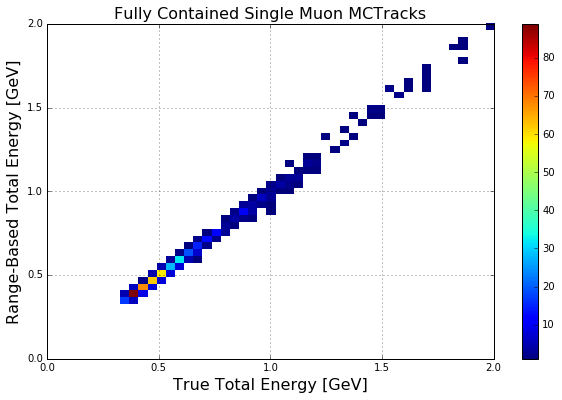
\includegraphics[width=100mm]{Figures/true_range_comparison_MCTracks.png}
\end{center}
\caption{\textit{Range based energy versus true energy for the single muon {\sc MCTrack} sample described in Section \ref{MCTrack_Selection_section}.}}
\label{true_range_energy_MCTrack_fig}
\end{figure}

\begin{figure}
\centering
\mbox{
	\subfigure[\textit{Fractional energy difference between 0.35 and 0.53 GeV true energy.}]
	{\includegraphics[width=50mm]{Figures/{true_range_resolution_SingleMuonMCTrack_slice_0.35_0.53}.png}}
	\quad
	\subfigure[\textit{Fractional energy difference between 0.90 and 1.08 GeV true energy.}]
	{\includegraphics[width=50mm]{Figures/{true_range_resolution_SingleMuonMCTrack_slice_0.90_1.08}.png}}
	\quad
	\subfigure[\textit{Fractional energy difference between 1.45 and 1.63 GeV true energy.}]
	{\includegraphics[width=50mm]{Figures/{true_range_resolution_SingleMuonMCTrack_slice_1.45_1.63}.png}}
	}
\caption{\textit{Fractional energy difference for a few representative bins of true energy derived from Figure \ref{true_range_energy_MCTrack_fig}.}}
\label{true_range_bias_resolution_MCTrack_slices_fig}
\end{figure}




\begin{figure}
\centering
\mbox{
	\subfigure[\textit{Range energy bias as a function of true energy. The vertical error bars are computed as $\frac{\sigma_{fit}}{\sqrt{N}}$, and the horizontal error bars indicate bin width.}]
	{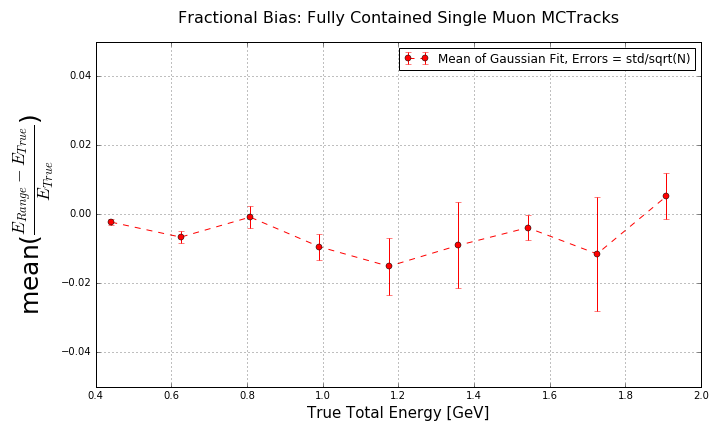
\includegraphics[width=75mm]{Figures/true_range_bias_SingleMuonMCTrack.png}}
	\quad
	\subfigure[\textit{Range energy resolution as a function of true energy. The vertical error bars are computed as $\frac{\sigma_{fit}}{\sqrt{2N}}$, and the horizontal error bars indicate bin width.}]
	{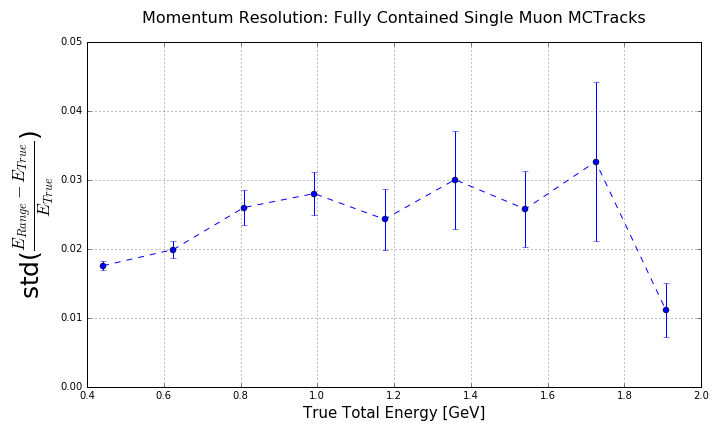
\includegraphics[width=75mm]{Figures/true_range_resolution_SingleMuonMCTrack.png}}
	}
\caption{\textit{Range energy and true energy bias and resolution for the single muon {\sc MCTrack} sample described in Section \ref{MCTrack_Selection_section}.}}
\label{true_range_bias_resolution_MCTrack_fig}
\end{figure}




\subsubsection{MCS Momentum Validation}\label{MCS_Momentum_Validation_MCTrack_section}
For this sample of {\sc MCTracks}, only the 3D trajectory points of each {\sc MCTrack} are used as input to the MCS code, described in Section \ref{MCS_technique_section}. The resulting MCS momentum versus range-based momentum can be seen in Figure \ref{MCS_range_momentum_MCTrack_fig}. Range momentum is used here instead of true momentum in order to make this plot more directly comparable with the same analysis on data where true momentum is not accessible. In order to compute a bias and a resolution, Figure \ref{MCS_range_momentum_MCTrack_fig} is sliced in bins of range momentum and a histogram of the fractional momentum difference ($\frac{p_{MCS}^{-1} - p_{range}^{-1}}{p_{range}^{-1}}$) is created for each bin. Note that the inverse of the momentum is used rather than the momentum because this distribution is more gaussian distributed. Also note that this fractional momentum difference using inverse of momentum is algebraically equivalent to ($\frac{p_{range} - p_{MCS}}{p_{MCS}}$). This distribution is shown for three representative bins in Figure \ref{MCS_range_bias_resolution_MCTrack_slices_fig}, along with the gaussian fit to each.  The mean ($\mu$) of each gaussian fit is used to compute a bias as a function of range momentum, while the width ($\sigma$) of each distribution is used to compute a resolution. The bias and resolution for this momentum reconstruction method shown in Figure \ref{MCS_range_bias_resolution_MCTrack_fig}. This figure indicates a bias in the MCS momentum resolution on the order of a few percent, with a resolution that decreases from about 9\% for contained {\sc MCTracks} with true total momentum around 0.5 GeV (which corresponds to a length of about 1.7 meters) to below 5\% for contained {\sc MCTracks} with true total momentum greater than 0.8 GeV (which corresponds to a length of about 3.1 meters).


\begin{figure}[ht!]
\begin{center}
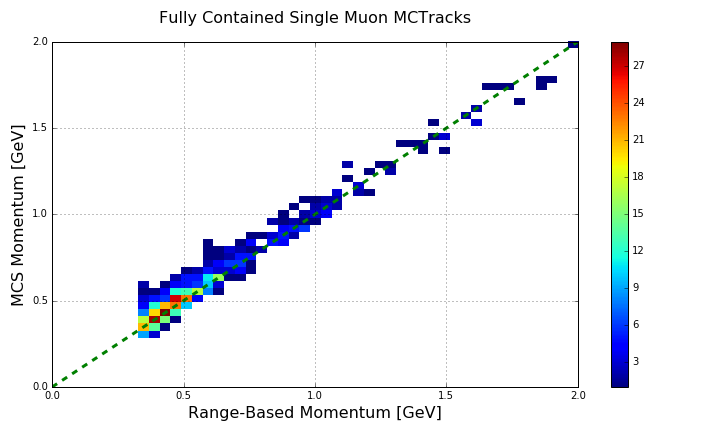
\includegraphics[width=100mm]{Figures/MCS_range_comparison_SingleMuonMCTrack.png}
\end{center}
\caption{\textit{MCS computed momentum versus range momentum for the single muon {\sc MCTrack} sample described in Section \ref{MCTrack_Selection_section}. Note the cutoff at around 0.3 GeV range-based momentum is caused by the minimum track length of 100 centimenter requirement.}}
\label{MCS_range_momentum_MCTrack_fig}
\end{figure}

\begin{figure}
\centering
\mbox{
	\subfigure[\textit{Fractional momentum difference between 0.35 and 0.53 GeV range momentum.}]
	{\includegraphics[width=50mm]{Figures/{MCS_range_resolution_SingleMuonMCTrack_slice_0.35_0.53}.png}}
	\quad
	\subfigure[\textit{Fractional momentum difference between 0.90 and 1.08 GeV true momentum.}]
	{\includegraphics[width=50mm]{Figures/{MCS_range_resolution_SingleMuonMCTrack_slice_0.90_1.08}.png}}
	\quad
	\subfigure[\textit{Fractional momentum difference between 1.45 and 1.63 GeV true momentum.}]
	{\includegraphics[width=50mm]{Figures/{MCS_range_resolution_SingleMuonMCTrack_slice_1.45_1.63}.png}}
	}
\caption{\textit{Fractional momentum difference for a few representative bins of range momentum derived from Figure \ref{MCS_range_momentum_MCTrack_fig}.}}
\label{MCS_range_bias_resolution_MCTrack_slices_fig}
\end{figure}


\begin{figure}
\centering
\mbox{
	\subfigure[\textit{MCS momentum bias as a function of range momentum. The vertical error bars are computed as $\frac{\sigma_{fit}}{\sqrt{N}}$, and the horizontal error bars indicate bin width.}]
	{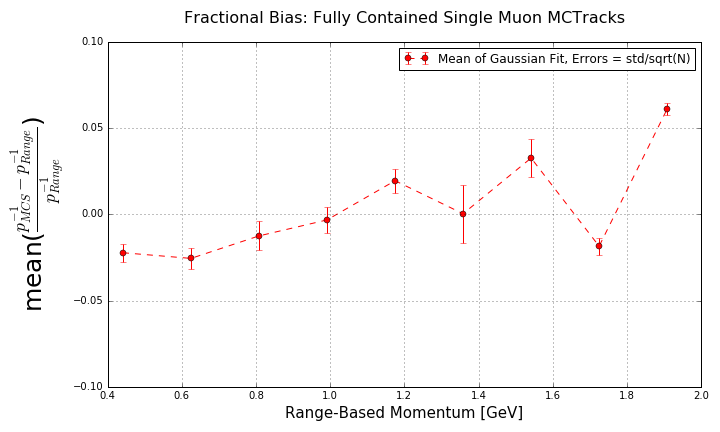
\includegraphics[width=75mm]{Figures/MCS_range_bias_SingleMuonMCTrack.png}}
	\quad
	\subfigure[\textit{MCS momentum resolution as a function of range momentum. The vertical error bars are computed as $\frac{\sigma_{fit}}{\sqrt{2N}}$, and the horizontal error bars indicate bin width.}]
	{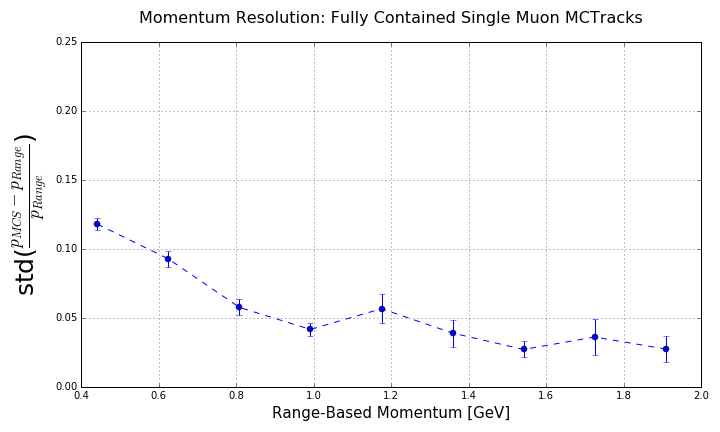
\includegraphics[width=75mm]{Figures/MCS_range_resolution_SingleMuonMCTrack.png}}
	}
\caption{\textit{MCS momentum bias and resolution as a function of range momentum for the single muon {\sc MCTrack} sample described in Section \ref{MCTrack_Selection_section}.}}
\label{MCS_range_bias_resolution_MCTrack_fig}
\end{figure}



\subsubsection{Highland Validation}\label{Highland_Validation_MCTrack_section}
For a given track segment momentum and length, 98\% of the angular scatter deviations should be gaussian with an RMS described by the Highland equation (Equation \ref{highland_eqtn}), while the remaining 2\% are larger angle Rutherford scatters\cite{highland}. Therefore, a histogram of track segment angular deviations divided by the RMS predicted by the Highland equation should be gaussian with a width of unity. In this section, we validate this claim.\\

For each 10 cm segment of each {\sc MCTrack} in this single muon sample, the momentum of the muon at the start of that segment is estimated by taking the computed MCS momentum and subtracting out momentum lost in the track upstream of the start of this segment, assuming the track was minimally ionizing as described in Equation \ref{segment_E_equation}. The segment momentum, along with the segment length, is converted into an expected RMS angular deviation by way of Equation \ref{highland_eqtn}. For each consecutive pair of segments, the angular scatter in milliradians divided by the Highland expected RMS in millradians is an entry in the histogram shown in Figure \ref{Highland_validation_MCTracks_fig}. From this figure we can see that the Highland formula is valid for {\sc MCTracks}, as the gaussian fit agrees well with the underlying histogram.

\begin{figure}[ht!]
\begin{center}
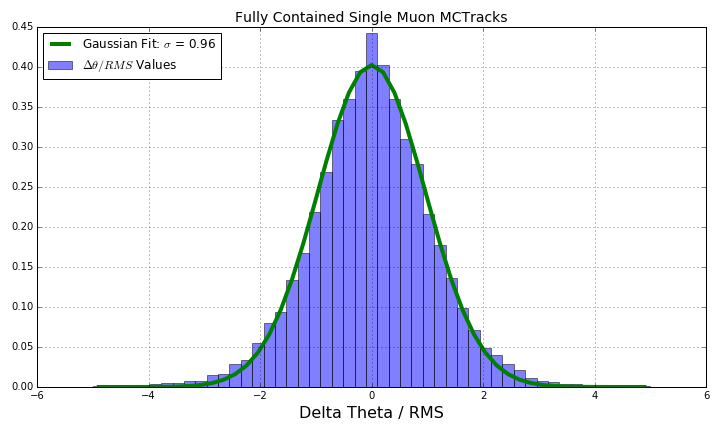
\includegraphics[width=100mm]{Figures/Highland_validation_SingleMuonMCTrack.png}
\end{center}
\caption{\textit{10 cm segment angular deviations divided by expected Highland RMS for the single muon {\sc MCTrack} sample described in Section \ref{MCTrack_Selection_section}.}}
\label{Highland_validation_MCTracks_fig}
\end{figure}













% %%%%%%%%%%%%%%%%%%%%%%%%%%%%%%%%%%%%%%%%%%%%%%%%%%%%%%%%%%%%%%%%%%%%%%%%%%%%%%%%%%%%%

% \subsection{Performance with Reconstructed Tracks}
% \subsubsection{Reconstructed Track Description}\label{RecoTrack_section}
% XXX this section has description of PandoraNuPMA tracks, cite pandora reference rather than lengthy description.

% \subsubsection{Reconstructed Track Selection}\label{RecoTrack_Selection_section}
% For analysis on single muon reconstructed tracks, the input sample is the one described in Section \ref{SingleMu_Input_Sample_section}. From that sample, the requirements described in Section \ref{MCTrack_Selection_section} are first placed on the sample. Then, the following additional requirements are placed for event selection:
% \begin{enumerate}
% 	\item There is exactly one reconstructed track in the event.
% 	\item The reconstructed track is longer than one meter in start-to-end length.
% 	\item The reconstructed track is fully contained within the fiducial volume (defined in Section \ref{fidvol_section}).
% 	\item The start of the reconstructed track is within 3 cm of the start of the {\sc MCTrack}, and the end of the reconstructed track is within 3c m of the end of the {\sc MCTrack} (or vice-versa).
% \end{enumerate}
% The last selection criteria is the one most worth noting; it ensures that the track is well reconstructed and not broken or truncated. The purpose the ``vice-versa'' clause in the last selection criteria is to take into account tracks that are well reconstructed in terms of position, but are flipped in direction. In the case of reverse-oriented tracks, the reconstructed track is flipped to have the correct direction before proceeding with the analysis. The application of these track selection cuts reduces the sample down to 307 reconstructed single muon tracks, which are used in this analysis.



% \subsubsection{MCS Energy Validation}\label{MCS_Energy_Validation_RecoTrack_section}
% For this sample of reconstructed tracks, only the trajectory points of each reconstructed track are used as input to the MCS code, described in Section \ref{MCS_technique_section}. The resulting MCS energy versus range-based energy can be seen in Figure \ref{MCS_range_energy_RecoTrack_fig}. In order to compute a bias and a resolution, Figure \ref{MCS_range_energy_RecoTrack_fig} is sliced in bins of range energy and a histogram of the fractional energy difference ($\frac{E_{MCS} - E_{range}}{E_{range}}$) is created for each bin. This distribution is shown for three representative bins in Figure \ref{MCS_range_bias_resolution_RecoTrack_slices_fig}. The mean of each distribution is used to compute a bias a function of range, while the standard deviation of each distribution is used to compute a resolution. The bias and resolution for this energy reconstruction method shown in Figure \ref{MCS_range_bias_resolution_RecoTrack_fig}. This figure indicates a bias in the MCS energy resolution on the order of a few percent, with a resolution that decreases from about 18\% for contained reconstructed tracks with range energy around 0.5 GeV (which corresponds to a length of about 1.7 meters) to below 10\% for contained reconstructed tracks with range energy greater than 0.8 GeV (which corresponds to a length of about 3.1 meters). This agrees very well with the same resolution and boas plots made for {\sc MCTracks} (Figure \ref{MCS_range_bias_resolution_MCTrack_fig}).


% \begin{figure}[ht!]
% \begin{center}
% 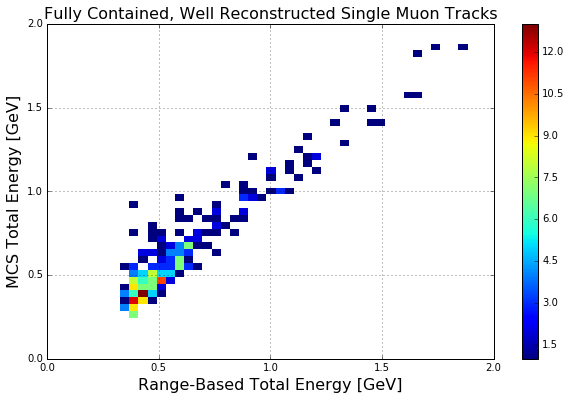
\includegraphics[width=100mm]{Figures/MCS_range_comparison_RecoTracks.png}
% \end{center}
% \caption{\textit{MCS computed energy versus range energy for the single muon reconstructed track sample described in Section \ref{RecoTrack_Selection_section}.}}
% \label{MCS_range_energy_RecoTrack_fig}
% \end{figure}

% \begin{figure}
% \centering
% \mbox{
% 	\subfigure[\textit{Fractional energy difference between 0.35 and 0.53 GeV range energy.}]
% 	{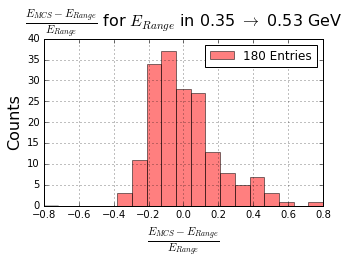
\includegraphics[width=50mm]{Figures/MCS_range_resolution_RecoTracks_slice1.png}}
% 	\quad
% 	\subfigure[\textit{Fractional energy difference between 0.90 and 1.08 GeV range energy.}]
% 	{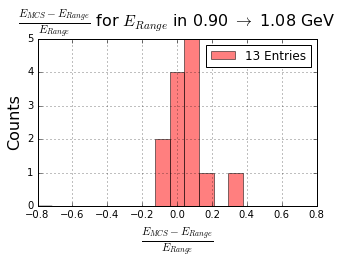
\includegraphics[width=50mm]{Figures/MCS_range_resolution_RecoTracks_slice2.png}}
% 	\quad
% 	\subfigure[\textit{Fractional energy difference between 1.45 and 1.63 GeV range energy.}]
% 	{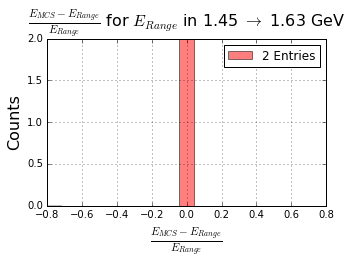
\includegraphics[width=50mm]{Figures/MCS_range_resolution_RecoTracks_slice3.png}}
% 	}
% \caption{\textit{Fractional energy difference for a few representative bins of range energy derived from Figure \ref{MCS_range_energy_RecoTrack_fig}.}}
% \label{MCS_range_bias_resolution_RecoTrack_slices_fig}
% \end{figure}


% \begin{figure}
% \centering
% \mbox{
% 	\subfigure[\textit{MCS energy bias as a function of range energy.}]
% 	{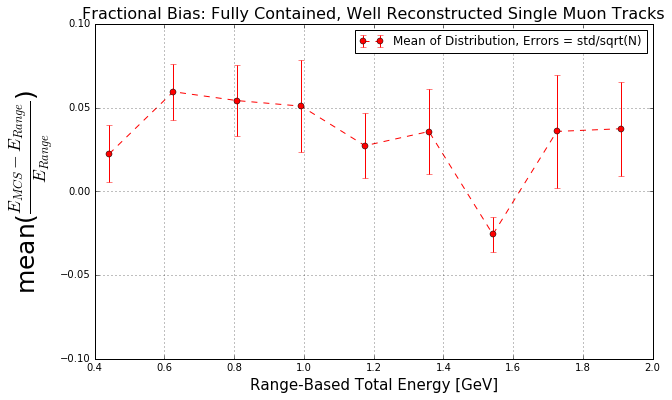
\includegraphics[width=75mm]{Figures/MCS_range_bias_RecoTracks.png}}
% 	\quad
% 	\subfigure[\textit{MCS energy resolution as a function of range energy.}]
% 	{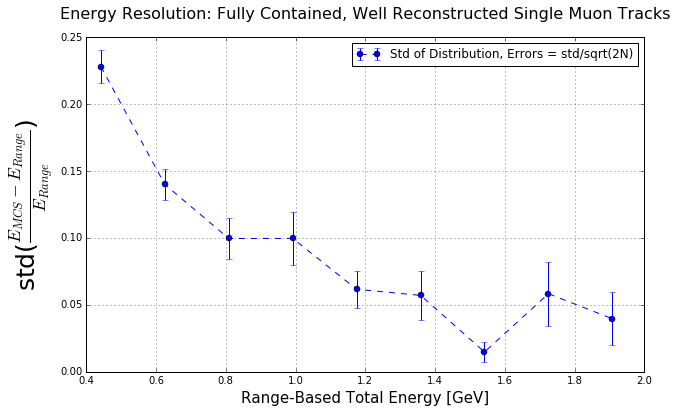
\includegraphics[width=75mm]{Figures/MCS_range_resolution_RecoTracks.png}}
% 	}
% \caption{\textit{MCS energy bias and resolution as a function of range energy for the single muon reconstructed track sample described in Section \ref{RecoTrack_Selection_section}.}}
% \label{MCS_range_bias_resolution_RecoTrack_fig}
% \end{figure}



% \subsubsection{Highland Validation}\label{Highland_Validation_RecoTrack_section}
% For this single muon reconstucted track sample, the same Highland validation plot is created in exactly the same way as described in Section \ref{Highland_Validation_MCTrack_section}. For each consecutive pairs of segments, the angular scatter in milliradians divided by the Highland expected RMS in millradians is an entry in the histogram shown in Figure \ref{Highland_validation_RecoTracks_fig}. From this figure we can see that the Highland formula is valid for reconstructed tracks, though the width is slightly smaller than unity. While the gaussian fit does not agree with the underlying histograms as it did in Section \ref{Highland_Validation_MCTrack_section} for {\sc MCTracks}, it is difficult to draw any conclusions about this plot due to extremely limited statistics. Instead the reader is referred to Section \ref{Highland_Validation_MCNuRecoTrack_section} which shows this plot for a higher statistic sample of simulated neutrino-induced muons which are contained.

% \begin{figure}[ht!]
% \begin{center}
% 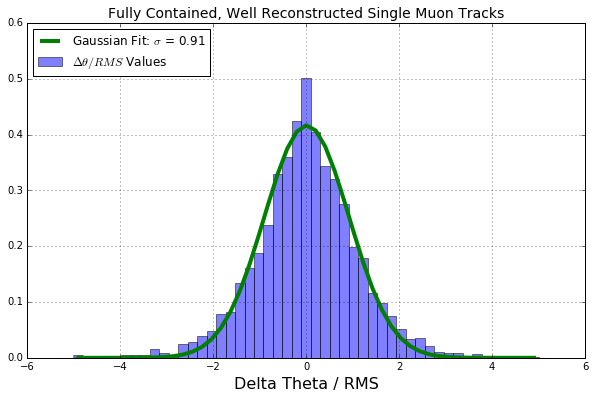
\includegraphics[width=100mm]{Figures/Highland_validation_RecoTracks.png}
% \end{center}
% \caption{\textit{20cm segment angular deviations divided by expected Highland RMS for the single muon reconstructed track sample described in Section \ref{RecoTrack_Selection_section}.}}
% \label{Highland_validation_RecoTracks_fig}
% \end{figure}


